% ==============================================================================
% Section 1.11: Epistemic Landscape and Open Problems
% ==============================================================================

\section{Epistemic Landscape and Consolidated Open Problems}
\label{sec:epistemic_map}

This section consolidates the epistemic status of all claims made in this chapter,
along with all open problems requiring future work. Rather than scattering ``What
Remains Open'' subsections throughout, we gather them here for clarity.

% =========================
% Part II — Book-ready box
% =========================
\begin{center}
\fbox{\parbox{0.94\linewidth}{
\textbf{Part II (Weak Sector) --- Status Map (as of 2026-01-22).}
\textit{PMNS angles:} $\theta_{23}$ \textbf{GREEN [Dc]} (Z$_6$ geometry);
$\theta_{13}$ \textbf{YELLOW [BL$\to$Dc]} via $\varepsilon=\lambda/\sqrt{2}$ (15\% off);
$\theta_{12}$ \textbf{YELLOW [Dc]} via $\arctan(1/\sqrt{2})$ (8.6\% off).
\textit{CKM CP:} Phase Cancellation Theorem \textbf{GREEN [Dc]} (pure Z$_3$ gives $J=0$);
Z$_2$ selection yields $\delta\simeq60^\circ$ \textbf{YELLOW [Dc]+[I]} (5° from PDG) with $J\simeq2.9\times10^{-5}$.
\textit{SU(2)$_L$:} minimal ``where/how'' embedding \textbf{YELLOW [P]} (brane-localized; $g_{\rm eff}\simeq g_2$ up to brane terms).
\textit{$G_F$:} sanity skeleton + \textbf{closure spine derived} ($G_F = g_5^2 \ell^2 I_4/x_1^2$ [Dc]; no-smuggling guardrails explicit); numeric closure \textbf{YELLOW [Dc]+[OPEN]} pending BVP.
\textbf{Hard blockers (P1):} OPR-02/21 thick-brane BVP (master key for $I_4$ + parity selection). \textit{(OPR-19/20/22 now have derivation spines [Dc].)}
}}
\end{center}

\marginpar{\footnotesize\textbf{Verdict (Part II):} Flavor numerics largely locked; gauge ``where/how'' fixed [P]; $G_F$ attack-surface mapped---true closure awaits BVP + $(g_5,m_\phi)$ from 5D first principles (no SM-circularity).}

\subsection{Quantitative Summary: Thresholds and Gates}

Before cataloging the epistemic status of each claim, we present the quantitative
data that underlies the case studies. This table is \textbf{not} EDC-specific;
it is baseline physics \tagBL{} that any framework must reproduce.

\subsubsection{Q-Gates and Kinematic Thresholds}

\begin{center}
\begin{tabular}{llccc}
\toprule
\textbf{Decay} & \textbf{Channel} & \textbf{$Q$-value} & \textbf{Gate} & \textbf{Status} \\
\midrule
\multirow{2}{*}{Neutron} & $n \to p + e^- + \bar\nu_e$ &
  $+0.782$ MeV & $\mathcal{P}_{\text{energy}}$ & OPEN \\
& $n \to p + \mu^- + \bar\nu_\mu$ &
  $-104.4$ MeV & $\mathcal{P}_{\text{energy}}$ & CLOSED \\
\addlinespace
\multirow{2}{*}{Muon} & $\mu^- \to e^- + \bar\nu_e + \nu_\mu$ &
  $+105.1$ MeV & $\mathcal{P}_{\text{energy}}$ & OPEN \\
& $\mu^- \to \text{hadrons}$ &
  --- & $\mathcal{P}_{\text{mode}}$ & FORBIDDEN \\
\addlinespace
\multirow{2}{*}{Tau} & $\tau^- \to e^-/\mu^- + \nu\bar\nu$ &
  $+1776/1671$ MeV & $\mathcal{P}_{\text{energy}}$ & OPEN \\
& $\tau^- \to \text{hadrons} + \nu_\tau$ &
  $+1637$ MeV & $\mathcal{P}_{\text{mode}}$ & OPEN \\
\addlinespace
\multirow{2}{*}{Pion} & $\pi^+ \to \mu^+ + \nu_\mu$ &
  $+33.9$ MeV & $\mathcal{P}_{\text{chir}}$ & OPEN \\
& $\pi^+ \to e^+ + \nu_e$ &
  $+139.1$ MeV & $\mathcal{P}_{\text{chir}}$ & SUPPRESSED \\
\addlinespace
Electron & $e^- \to X$ & --- & No lower mode & BLOCKED \\
\bottomrule
\end{tabular}
\end{center}

\paragraph{Reading the table.}
\begin{itemize}[nosep]
  \item $Q > 0$: kinematically allowed (energy available for products)
  \item $Q < 0$: kinematically forbidden (would violate energy conservation)
  \item SUPPRESSED: allowed but with reduced amplitude (helicity suppression)
  \item FORBIDDEN: blocked by mode mismatch, not kinematics
  \item BLOCKED: no decay channel exists
\end{itemize}

\subsubsection{Mass and Lifetime Data}

\begin{center}
\begin{tabular}{lcccc}
\toprule
\textbf{Particle} & \textbf{Mass (MeV)} & \textbf{Lifetime} &
\textbf{Ontology} & \textbf{Dominant Gate} \\
\midrule
Neutron & $939.565$ & $879.4$ s & Bulk-core junction &
$\mathcal{P}_{\text{energy}}$ \\
Muon & $105.66$ & $2.20~\mu$s & Brane-dominant &
$\mathcal{P}_{\text{mode}}$ \\
Tau & $1776.9$ & $0.290$ ps & Brane-dominant &
$\mathcal{P}_{\text{energy}}$ \\
Pion & $139.57$ & $26.0$ ns & Junction-pair &
$\mathcal{P}_{\text{chir}}$ \\
Electron & $0.511$ & $> 10^{28}$ yr & Brane defect (ground) &
None (stable) \\
Neutrino & $< 10^{-6}$ & Stable & Edge mode &
Overlap suppression \\
\bottomrule
\end{tabular}
\end{center}

All values are \tagBL{} (PDG 2024). The ``Ontology'' and ``Dominant Gate'' columns
are EDC interpretations \tagP{}/\tagDc{}.

\subsubsection{What the Table Shows}

This quantitative summary demonstrates that:
\begin{enumerate}[nosep]
  \item \textbf{Channel selection is kinematic}: Neutron $\to$ electron (not muon)
        because $Q_\beta(\mu) < 0$.
  \item \textbf{Mode overlap matters}: Muon $\to$ leptons only because mode mismatch
        forbids hadronic channels.
  \item \textbf{Chirality suppression is real}: Pion $\to$ muon dominates over
        electron by $(m_\mu/m_e)^2 \approx 4 \times 10^4$.
  \item \textbf{Electron stability is structural}: No lower charged mode exists.
\end{enumerate}

These are \emph{facts} that EDC must be consistent with; they are not EDC-derived
claims.

\vspace{1em}

This section provides a comprehensive summary of the epistemic status of each
claim made in this chapter. The goal is transparency: the reader should know
exactly what is established, what is structural interpretation, and what
remains to be computed.

\subsection{The Five Categories}

Throughout this chapter, we have used the following epistemic tags:

\begin{center}
\begin{tabular}{clp{8cm}}
\toprule
\textbf{Tag} & \textbf{Status} & \textbf{Meaning} \\
\midrule
\tagBL{} & Baseline & Established experimental fact or Standard Model result \\
 & Definition & Terminological convention adopted in this work \\
\tagP{} & Postulate & Structural assumption or hypothesis \\
\tagDc{} & Deduction & Derived from postulates via explicit reasoning \\
(open) & Open & Requires further work; not yet computed or proven \\
\bottomrule
\end{tabular}
\end{center}

\subsection{Baseline Facts (What We Must Reproduce)}

The following are empirical facts that EDC must be consistent with:

\subsubsection{Particle Properties}

\begin{center}
\begin{tabular}{lll}
\toprule
\textbf{Quantity} & \textbf{Value} & \textbf{Source} \\
\midrule
Neutron mass & $m_n = 939.565$ MeV & PDG \\
Proton mass & $m_p = 938.272$ MeV & PDG \\
Electron mass & $m_e = 0.511$ MeV & PDG \\
Muon mass & $m_\mu = 105.66$ MeV & PDG \\
Tau mass & $m_\tau = 1776.9$ MeV & PDG \\
Pion mass & $m_{\pi^\pm} = 139.57$ MeV & PDG \\
\bottomrule
\end{tabular}
\end{center}

\subsubsection{Lifetimes}

\begin{center}
\begin{tabular}{lll}
\toprule
\textbf{Particle} & \textbf{Lifetime} & \textbf{Source} \\
\midrule
Neutron & $\tau_n \approx 880$ s & PDG \\
Muon & $\tau_\mu \approx 2.2 \times 10^{-6}$ s & PDG \\
Tau & $\tau_\tau \approx 2.9 \times 10^{-13}$ s & PDG \\
Pion & $\tau_\pi \approx 2.6 \times 10^{-8}$ s & PDG \\
Electron & $> 10^{28}$ years & PDG (limit) \\
\bottomrule
\end{tabular}
\end{center}

\subsubsection{Decay Channels and Branching Ratios}

\begin{center}
\begin{tabular}{lll}
\toprule
\textbf{Decay} & \textbf{Branching Ratio} & \textbf{Status} \\
\midrule
$n \to p + e^- + \bar\nu_e$ & $\approx 100\%$ & \tagBL{} \\
$\mu^- \to e^- + \bar\nu_e + \nu_\mu$ & $\approx 100\%$ & \tagBL{} \\
$\tau^- \to e^- + \bar\nu_e + \nu_\tau$ & $\approx 17.8\%$ & \tagBL{} \\
$\tau^- \to \mu^- + \bar\nu_\mu + \nu_\tau$ & $\approx 17.4\%$ & \tagBL{} \\
$\tau^- \to \text{hadrons} + \nu_\tau$ & $\approx 64.8\%$ & \tagBL{} \\
$\pi^+ \to \mu^+ + \nu_\mu$ & $\approx 99.99\%$ & \tagBL{} \\
$\pi^+ \to e^+ + \nu_e$ & $\approx 0.012\%$ & \tagBL{} \\
\bottomrule
\end{tabular}
\end{center}

\subsubsection{Coupling Constants}

\begin{center}
\begin{tabular}{lll}
\toprule
\textbf{Quantity} & \textbf{Value} & \textbf{Source} \\
\midrule
Fermi constant & $G_F = 1.166 \times 10^{-5}~\text{GeV}^{-2}$ & PDG \\
$W$ boson mass & $M_W = 80.4$ GeV & PDG \\
Fine structure const. & $\alpha \approx 1/137$ & CODATA \\
\bottomrule
\end{tabular}
\end{center}

\subsection{Postulates (Structural Assumptions)}

The following are hypotheses that define the EDC framework:

\begin{center}
\begin{tabular}{p{4cm}p{9cm}}
\toprule
\textbf{Postulate} & \textbf{Statement} \\
\midrule
Thick brane & The 3D universe is a finite-thickness layer in 5D \\
Bulk-core particles & Neutron, proton have 5D bulk structure \\
Brane-dominant modes & Leptons are excitations of the brane layer \\
Edge modes & Neutrinos are localized at the bulk-brane interface \\
Frozen projection & Observer-facing boundary is quasi-static \\
Pipeline structure & Weak decays proceed via absorption-dissipation-release \\
Mode overlap & Branching ratios depend on wavefunction overlaps \\
Chirality projection & Boundary conditions select helicity \\
\bottomrule
\end{tabular}
\end{center}

\subsection{Deductions (What Follows from Postulates)}

The following claims are derived from the postulates:

\subsubsection{Qualitative Deductions}

\begin{center}
\begin{tabular}{p{5cm}p{8cm}}
\toprule
\textbf{Claim} & \textbf{Derivation Path} \\
\midrule
Neutron decays to electron (not muon) & Kinematic threshold: $Q_\beta(\mu) < 0$ \\
Electron is stable & No lower-lying charged mode exists \\
Muon decay is purely leptonic & Mode mismatch with hadrons \\
Tau has hadronic channels & Higher mode energy opens thresholds \\
Neutrinos interact weakly & Edge-mode localization suppresses overlap \\
\bottomrule
\end{tabular}
\end{center}

\subsubsection{Quantitative Deductions}

\begin{center}
\begin{tabular}{p{4cm}p{5cm}p{4cm}}
\toprule
\textbf{Quantity} & \textbf{EDC Expression} & \textbf{Status} \\
\midrule
$Q_\beta(e)$ value & $m_n - m_p - m_e = 0.782$ MeV & \tagDc{} (arithmetic) \\
$Q_\beta(\mu)$ sign & $< 0$ (channel closed) & \tagDc{} \\
$R_{e/\mu}$ scaling & $\propto (m_e/m_\mu)^2$ & \tagBL{} + \tagP{} \\
\bottomrule
\end{tabular}
\end{center}

\subsection{Open Problems (What Remains to Be Done)}

The following require further work:

\subsubsection{Critical Open Problems}

\begin{center}
\begin{tabular}{p{5cm}p{8cm}}
\toprule
\textbf{Problem} & \textbf{What Is Needed} \\
\midrule
Neutron lifetime value & Compute tunneling rate from 5D junction dynamics \\
$G_F$ derivation & Compute overlap integral in thick-brane background \\
Helicity suppression factor & Solve Dirac equation with boundary conditions \\
Mode spectrum & Solve thick-brane eigenvalue problem \\
Neutrino mass & Compute edge-mode energy \\
\bottomrule
\end{tabular}
\end{center}

\subsubsection{Important but Non-Critical}

\begin{center}
\begin{tabular}{p{5cm}p{8cm}}
\toprule
\textbf{Problem} & \textbf{What Is Needed} \\
\midrule
Tau branching ratios & Compute mode overlaps for hadronic channels \\
$\mu/\tau$ lifetime ratio & Connect to mode energy differences \\
Generation structure & Explain three lepton generations from geometry \\
Neutrino mixing ($\theta_{12}$, $\theta_{13}$) & Structure identified (Attempt~4); geometric origin of $\theta_{12}^0$, $\varepsilon$ needed \\
\bottomrule
\end{tabular}
\end{center}

\subsection{Visual Summary: The Epistemic Landscape}

\begin{center}
\begin{tikzpicture}[scale=0.9]

% Baseline region
\fill[green!15] (-5,0) rectangle (5,1.5);
\node[font=\small\bfseries, green!50!black] at (0,1.2) {BASELINE (Established)};
\node[font=\scriptsize, align=center] at (-2.5,0.5) {Masses, lifetimes,\\branching ratios};
\node[font=\scriptsize, align=center] at (2.5,0.5) {$G_F$, $M_W$,\\SM formulas};

% Postulate region
\fill[yellow!20] (-5,1.7) rectangle (5,3.2);
\node[font=\small\bfseries, yellow!60!black] at (0,2.9) {POSTULATES (Structural Assumptions)};
\node[font=\scriptsize, align=center] at (-2.5,2.2) {Thick brane,\\bulk-core particles};
\node[font=\scriptsize, align=center] at (2.5,2.2) {Frozen projection,\\pipeline structure};

% Deduction region
\fill[blue!15] (-5,3.4) rectangle (5,4.9);
\node[font=\small\bfseries, blue!50!black] at (0,4.6) {DEDUCTIONS (Derived from Postulates)};
\node[font=\scriptsize, align=center] at (-2.5,3.9) {Channel selection,\\stability conditions};
\node[font=\scriptsize, align=center] at (2.5,3.9) {Qualitative patterns,\\threshold effects};

% Open region
\fill[red!10] (-5,5.1) rectangle (5,6.6);
\node[font=\small\bfseries, red!50!black] at (0,6.3) {OPEN (To Be Computed)};
\node[font=\scriptsize, align=center] at (-2.5,5.6) {Lifetime values,\\$G_F$ derivation};
\node[font=\scriptsize, align=center] at (2.5,5.6) {Mode spectrum,\\overlap integrals};

% Arrows showing logical flow
\draw[-{Stealth}, thick, gray] (5.5,0.75) -- (5.5,2.45);
\draw[-{Stealth}, thick, gray] (5.5,2.45) -- (5.5,4.15);
\draw[-{Stealth}, thick, gray] (5.5,4.15) -- (5.5,5.85);
\node[font=\tiny, rotate=90] at (5.9,3.3) {logical dependence};

\end{tikzpicture}
\end{center}

\subsection{What This Chapter Does and Does Not Claim}

\begin{tcolorbox}[readerContract, title={Final Epistemic Statement}]
\textbf{This chapter claims}:
\begin{itemize}[nosep]
  \item A coherent structural interpretation of weak decays in thick-brane geometry
  \item Qualitative explanations for channel selection rules
  \item A well-posed framework for quantitative computation
  \item Explicit falsifiability conditions for each claim
\end{itemize}

\textbf{This chapter does not claim}:
\begin{itemize}[nosep]
  \item First-principles derivation of lifetime values
  \item Explicit computation of branching ratios
  \item Derivation of $G_F$ from the 5D action
  \item Complete solution of the mode spectrum
\end{itemize}

The gap between ``structural interpretation'' and ``derived result'' is
substantial. Closing this gap is the research program.
\end{tcolorbox}

\vspace{0.5em}
\noindent\textit{For readers who want a forensic trail (what was tested, what was rejected,
and which equations support it), a supplementary \textbf{Meta Documentation Pack} for Part~II
contains a Claim Ledger, Decision Log, Research Timeline, and Evidence Map, and can be
optionally included at compile time.}

% ==============================================================================
\subsection{Open Problems Register (OPR)}
\label{sec:opr}

\begin{tcolorbox}[colback=yellow!4, colframe=yellow!60!black,
    title=\textbf{Open Status (Part II)}]
\textbf{Part~II is not closed.} The weak-sector narrative is now internally
consistent, but several results remain explicitly \emph{open}: (i)~full
$\mathrm{SU}(2)_L$ embedding, (ii)~PMNS angles beyond the $\mathbb{Z}_3$
baseline, (iii)~the CKM apex $(\bar\rho, \bar\eta)$ and a $\delta$ refinement
beyond the discrete-phase estimate, and (iv)~a first-principles bridge for
$(g_5, m_\phi)$ and the BVP/KK spectrum. These are tracked in the Open
Problems Register and addressed as a staged research program.
\end{tcolorbox}

\subsubsection{Priority-1 Open Problems}

The following items block major claims and define the immediate research program:

\begin{table}[ht]
\centering
\caption{Open Problems Register: Priority-1 items}
\label{tab:opr_p1}
\begin{tabular}{lp{5cm}lp{4cm}}
\toprule
\textbf{ID} & \textbf{Item} & \textbf{Status} & \textbf{Next Action} \\
\midrule
OPR-02 & KK tower truncation (N$_{\text{gen}}$) & RED-C [P] & BVP Work Package (\S\ref{sec:ch12_bvp_workpackage}) \\
OPR-05a & PMNS $\theta_{23}$ & \textcolor{OliveGreen}{\textbf{GREEN}} [Dc] & Closed: $\sin^2\theta_{23} = 0.564$ (3\%) \\
OPR-05b & PMNS $\theta_{13}$/ε & \textcolor{YellowOrange}{\textbf{YELLOW}} [BL$\to$Dc] & $\varepsilon = \lambda/\sqrt{2}$, 15\% from PDG \\
OPR-05c & PMNS $\theta_{12}$ & \textcolor{YellowOrange}{\textbf{YELLOW}} [Dc] & $\arctan(1/\sqrt{2}) = 35.26°$ (8.6\% off) \\
OPR-11 & CKM $(\bar\rho, \bar\eta)$ & \textcolor{YellowOrange}{\textbf{YELLOW}} [Dc]+[P] & Odd sign-flip rule [Dc]; brane-parity [P]; BVP needed \\
OPR-12 & CP phase $\delta$ & \textcolor{YellowOrange}{\textbf{YELLOW}} [Dc]+[I] & $\delta = 60°$ (5° from PDG); Phase Cancellation Thm \\
OPR-17 & SU(2)$_L$ gauge embedding & \textcolor{YellowOrange}{\textbf{YELLOW}} [P] & Where/how fixed; origin+masses OPEN \\
OPR-22 & $G_F$ first-principles & \textcolor{YellowOrange}{\textbf{YELLOW}} [Dc]+[OPEN] & Closure spine [Dc]; no-smuggling guardrails; numerics [OPEN] \\
\bottomrule
\end{tabular}
\end{table}

\subsubsection{State of Play by Sector}

\paragraph{CKM/CP (Chapter~\ref{sec:ch7_ckm}).}
\begin{itemize}[nosep]
    \item \textcolor{OliveGreen}{\textbf{Closed:}} Magnitude hierarchy $\lambda$, $\lambda^2$, $\lambda^3$ from overlap localization \tagDc{}
    \item \textcolor{OliveGreen}{\textbf{Closed:}} Phase Cancellation Theorem: pure $\mathbb{Z}_3$ gives $J = 0$ \tagDc{}
    \item \textcolor{YellowOrange}{\textbf{Partial:}} $\delta = 60°$ (5° from PDG) via $\mathbb{Z}_2$ sign selection; $J = 2.9 \times 10^{-5}$ (6\%) \tagDc{}+\tagI{}
    \item \textcolor{YellowOrange}{\textbf{Partial:}} $\mathbb{Z}_2$ parity: odd sign-flip rule \tagDc{}, brane-reflection parity \tagP{}; specific element (BVP) open
    \item \textcolor{BrickRed}{\textbf{Open:}} BVP profile parities; residual 5° in $\delta$
\end{itemize}

\paragraph{PMNS/Neutrinos (Chapter~\ref{sec:ch6_pmns}).}
\begin{itemize}[nosep]
    \item \textcolor{OliveGreen}{\textbf{Closed:}} DFT baseline falsified; $\theta_{23} \approx 45°$ derived from $\mathbb{Z}_6$ geometry (3\% accuracy) \tagDc{}
    \item \textcolor{YellowOrange}{\textbf{Partial:}} $\varepsilon = \lambda/\sqrt{2}$ (Attempt~4.1) predicts reactor scale (15\%); $\theta_{12} = \arctan(1/\sqrt{2})$ (Attempt~4.2) provides geometric origin (8.6\%)---both [Dc], no PDG-smuggling
    \item \textcolor{BrickRed}{\textbf{Open:}} CP phase; Dirac vs Majorana; T1 vs T2 selection for $\theta_{12}$
\end{itemize}

\paragraph{$G_F$ and Weak Coupling (Chapter~\ref{sec:gf_pathway}).}
\begin{itemize}[nosep]
    \item \textcolor{OliveGreen}{\textbf{Closed:}} Numerical pathway consistent with EW relations \tagDc{}
    \item \textcolor{OliveGreen}{\textbf{Closed:}} Canonical $g_5$ normalization: $g_4 = g_5$ with orthonormal modes \tagDc{}
    \item \textcolor{OliveGreen}{\textbf{Closed:}} KK spectrum form: $m_\phi = x_1/\ell$ from eigenvalue equation \tagDc{}
    \item \textcolor{YellowOrange}{\textbf{Partial:}} Mode overlap mechanism identified \tagP{}
    \item \textcolor{YellowOrange}{\textbf{Partial:}} Closure spine: $G_F = g_5^2 \ell^2 I_4 / x_1^2$ \tagDc{}; no-smuggling guardrails explicit
    \item \textcolor{BrickRed}{\textbf{Open:}} $g_5$ value; $\ell$ from membrane; exact BVP solutions for $I_4$
\end{itemize}

\subsubsection{Highest-Value Closure Targets}

\begin{enumerate}
    \item \textbf{Thick-brane BVP solver} --- appears in 5 OPR items; unlocks generation
          counting, pion decay, $G_F$ derivation, neutrino masses
    \item \textbf{CP mechanism refinement} --- appears in 4 OPR items; Z$_6$ = Z$_2 \times$ Z$_3$
          analysis may close both CKM and PMNS phase sectors
    \item \textbf{KK reduction} --- needed for $g_5$, $m_\phi$; quantitative $G_F$
\end{enumerate}

\paragraph{Philosophy.}
Open problems are not weaknesses---they are precisely enumerated targets for future
work. A theory with well-defined gaps is stronger than one with hidden assumptions.
The OPR ensures that every ``(open)'' marker in this text has a tracking entry,
a priority, and a concrete next action.

\subsubsection{OPR Closure Plan}

\begin{tcolorbox}[colback=blue!5, colframe=blue!60!black,
    title=\textbf{OPR Closure Plan: Prioritized Research Program}]
The following staged approach addresses OPR items in order of maximum payoff:

\textbf{P1-A: CP Sector Closure (OPR-06, OPR-11, OPR-12)}
\begin{itemize}[nosep]
    \item \emph{Status:} Attempt~4 + Z$_2$ parity origin completed; $\delta = 60°$ (5° from PDG); OPR-11 upgraded to YELLOW [Dc]+[P]
    \item \emph{Closed:} Odd sign-flip rule \tagDc{}; brane-reflection parity mechanism \tagP{}
    \item \emph{Remaining:} Specific element ($V_{cb}$ or $V_{ub}$) from BVP profile parities; residual 5° in $\delta$
    \item \emph{Payoff:} CKM sector structurally closed; PMNS CP phase (OPR-06) uses same $\mathbb{Z}_6$ framework
\end{itemize}

\textbf{P1-B: PMNS Mixing (OPR-05a/b/c, OPR-08) --- ALL ANGLES GEOMETRIC}
\begin{itemize}[nosep]
    \item \emph{Status:} Attempts~2--4.2 completed; all three angles now have geometric mechanisms, none calibrated to PDG
    \item \emph{Result (Attempt~2):} $\theta_{23}$ GREEN (3\%) from $\mathbb{Z}_6$ geometry \tagDc{}
    \item \emph{Result (Attempt~3):} Discrete $\mathbb{Z}_6$ phases insufficient for $\theta_{12}$, $\theta_{13}$
    \item \emph{Result (Attempt~4):} Rank-2 structure $U = R_{23} \cdot R_{13}(\varepsilon) \cdot R_{12}$ achieves GREEN
    \item \emph{Result (Attempt~4.1):} $\varepsilon = \lambda/\sqrt{2}$ predicts $\sin^2\theta_{13} = 0.025$ (15\% from PDG) \emph{without fitting} [BL$\to$Dc]
    \item \emph{Result (Attempt~4.2):} $\theta_{12} = \arctan(1/\sqrt{2}) = 35.26°$ provides geometric origin ($8.6\%$ from PDG) \tagDc{}---unified $\sqrt{2}$ factor with $\varepsilon$
    \item \emph{Key insight:} Same $\sqrt{2}$ appears in both $\varepsilon$ and $\theta_{12}$---suggests unified geometric origin
    \item \emph{Remaining:} Selection rule T1 vs T2; CP phase
\end{itemize}
\noindent\fbox{\parbox{0.96\textwidth}{\small
\textbf{PMNS closure:} OPR-05a GREEN ($\theta_{23}$ from $\mathbb{Z}_6$, 3\%), OPR-05b YELLOW ($\varepsilon = \lambda/\sqrt{2} \to \theta_{13}$, 15\%), OPR-05c YELLOW ($\theta_{12} = \arctan(1/\sqrt{2})$, 8.6\%)---all geometric [Dc], none calibrated to PDG.}}

\textbf{P1-C: Thick-Brane BVP (OPR-02, OPR-09, OPR-14, OPR-21) --- WORK PACKAGE DEFINED}
\begin{itemize}[nosep]
    \item \emph{Status:} BVP Work Package defined (\S\ref{sec:ch12_bvp_workpackage}); solver skeleton demonstrates bound states; acceptance criteria + failure modes documented
    \item \emph{Established:} Dimensionless BVP formulation; $I_4$ overlap integral computed; grid convergence for Neumann/Mixed BCs
    \item \emph{Open:} Physical potential $V(z)$ from membrane params $(\sigma, r_e)$; BC justification from physics
    \item \emph{Payoff:} Unlocks generation counting, mode profiles, overlap integrals
\end{itemize}

\textbf{P2: $G_F$ Chain (OPR-19--22) --- CLOSURE SPINE DERIVED [Dc]+[OPEN]}
\begin{itemize}[nosep]
    \item \emph{Status:} Full closure plan complete (\S\ref{sec:ch11_full_closure}); \textbf{OPR-22 upgraded to YELLOW [Dc]+[OPEN]}
    \item \emph{Closed:} Closure spine $G_F = g_5^2 \ell^2 I_4 / x_1^2$ [Dc]; no-smuggling guardrails; attack-surface map
    \item \emph{Closed (earlier):} $g_4 = g_5$ canonical normalization [Dc]; $m_\phi = x_1/\ell$ KK form [Dc]
    \item \emph{Open:} $g_5$ value (OPR-19); $\ell$ from membrane (OPR-20); $I_4$ from BVP profiles (OPR-21)
    \item \emph{Payoff:} First-principles $G_F$ without SM circularity---framework non-circular by construction
\end{itemize}
\noindent\emph{G$_F$ chain:} OPR-19/20/22 now have derivation spines [Dc]. Only BVP numerics (OPR-21) + underlying $g_5$ remain. True independent prediction is $\sin^2\theta_W = 1/4$; numerical $G_F$ uses SM relations (consistency, not derivation). No hidden tuning.

\textbf{P3: Gauge Structure (OPR-17) --- WHERE/HOW FIXED}
\begin{itemize}[nosep]
    \item \emph{Status:} YELLOW [P] --- Brane-localized SU(2)$_L$ embedding; overlap coupling $g_{\text{eff}} \simeq g_2$
    \item \emph{Closed:} Where gauge fields live (boundary); how they couple (overlap integral)
    \item \emph{Open:} Gauge symmetry origin; W$^\pm$/Z$^0$ mass generation
    \item \emph{Next:} Derive why SU(2)$_L$ symmetry exists; Higgs mechanism in 5D
\end{itemize}

\textbf{Summary:} 24 OPR items total. P1 items (A+B+C) close flavor physics.
P2 closes weak coupling quantitatively. P3 completes gauge structure.
\end{tcolorbox}

% ==============================================================================
% BVP WORK PACKAGE: Infrastructure for OPR-02/21 closure
% ==============================================================================
%!TEX root = ../EDC_Part_II_Weak_Sector.tex
% ==============================================================================
% BVP Work Package: Thick-Brane Solver Specification (OPR-02/21)
% Status: Infrastructure definition — NOT claiming closure
% ==============================================================================

\section{BVP Work Package: Thick-Brane Solver Specification}
\label{sec:ch12_bvp_workpackage}

% ------------------------------------------------------------------------------
% EPISTEMIC STATUS BOX
% ------------------------------------------------------------------------------

\begin{tcolorbox}[edcGuardrail, title=\textbf{Epistemic Status}]
This chapter defines \textbf{infrastructure}---not closure. It specifies the
mathematical problem that must be solved to close OPR-02/21.

\textbf{IF (Postulates) \tagP{}:}
\begin{itemize}[nosep]
    \item The 5D profile equation has Schrödinger form (Eq.~\eqref{eq:bvp_schrodinger})
    \item Potential shape $V(\xi)$ comes from membrane geometry (ansatz, not derived)
    \item Boundary conditions reflect brane microphysics (choice, not derived)
\end{itemize}

\textbf{THEN (Derived-conditional) \tagDc{}:}
\begin{itemize}[nosep]
    \item Dimensionless reduction is pure mathematics (no physics content)
    \item Sturm--Liouville structure guarantees discrete eigenvalues (if $V$ is confining)
    \item Overlap integrals $I_4$ are well-defined once profiles exist
\end{itemize}

\textbf{OPEN:}
\begin{itemize}[nosep]
    \item Derive $V(\xi)$ from $(\sigma, r_e)$ membrane parameters
    \item Derive boundary conditions from junction physics (Robin from Israel matching?)
    \item Connect eigenvalue spectrum to generation counting (OPR-02)
\end{itemize}

\textbf{Key distinction:} This chapter provides the \emph{recipe}, not the \emph{meal}.
All numerical outputs from the skeleton are \emph{sanity checks}, not predictions.
\end{tcolorbox}

% ==============================================================================
% FRAMEWORK 2.0 LANGUAGE COMPLIANCE
% ==============================================================================
\begin{tcolorbox}[colback=blue!3!white, colframe=blue!50!black,
    title=\textbf{Framework 2.0 Language Compliance}]
\small
\textbf{EDC Projection Principle:} Every physical process has a \textbf{5D bulk+brane cause}
whose observable residue is a \textbf{3D shadow} on the observer boundary.

\textbf{In this chapter:}
\begin{itemize}[nosep]
    \item \textbf{5D cause:} Thick-brane profile $f(\xi)$ governed by effective potential $V(\xi)$.
    \item \textbf{Brane process:} Boundary value problem determines eigenvalue spectrum.
    \item \textbf{3D shadow:} Particle masses, overlap integrals, effective couplings.
\end{itemize}

\textbf{The BVP is the mathematical engine} that translates 5D geometry into 3D observables.
Solving it is prerequisite for non-circular predictions.
\end{tcolorbox}

% ------------------------------------------------------------------------------

This subsection defines a \textbf{Work Package} for the thick-brane boundary value
problem (BVP) that appears in multiple OPR items. The goal is infrastructure, not
closure: define the problem precisely, establish acceptance criteria, and provide
a minimal solver skeleton for future development.

\begin{tcolorbox}[colback=yellow!5!white, colframe=yellow!60!black,
    title=\textbf{Scope Limitation}]
This work package does \textbf{not} claim to:
\begin{itemize}[nosep]
    \item Derive generation counting (OPR-02)
    \item Close CKM/PMNS from first principles
    \item Provide complete $G_F$ derivation
\end{itemize}
It \textbf{does} provide:
\begin{itemize}[nosep]
    \item Precise mathematical specification of the BVP
    \item Acceptance criteria for ``success''
    \item Failure modes and their implications
    \item Minimal numerical skeleton for testing
\end{itemize}
\end{tcolorbox}

% ------------------------------------------------------------------------------
% PHYSICAL PROCESS NARRATIVE
% ------------------------------------------------------------------------------

\begin{tcolorbox}[colback=green!5!white, colframe=green!50!black,
    title=\textbf{Physical Process Narrative: From Brane Thickness to Effective Couplings}]
\textbf{What physically happens, step by step:}

\textbf{Step 1: The brane has finite thickness.}
In EDC, the 3D universe is not an infinitely thin membrane but a \emph{thick layer}
of width $\Delta \sim r_e \sim 1$ fm embedded in the 5D bulk. This thickness is
physical---it sets the scale for localization \tagP{}.

\textbf{Step 2: Particles are ``standing waves'' in the extra dimension.}
A 4D particle (electron, quark) corresponds to a profile $f(\xi)$ in the 5th dimension.
Think of it as a guitar string clamped at both ends: only certain wavelengths fit,
giving discrete allowed masses \tagP{}.

\textbf{Step 3: The profile equation is Schrödinger-like.}
The 5D Dirac equation, after dimensional reduction, yields:
$[-d^2/d\xi^2 + V(\xi)]f = m^2 f$. This is a 1D quantum mechanics problem with $V(\xi)$
as the effective potential from brane geometry \tagDc{}.

\textbf{Step 4: The potential shape determines the spectrum.}
A deep well gives tightly localized modes (small overlap, weak coupling).
A shallow well gives extended modes (large overlap, strong coupling).
The number of bound states determines how many ``generations'' exist \tagDc{}.

\textbf{Step 5: Normalization fixes the coupling strength.}
If $f(\xi)$ is normalized ($\int |f|^2 d\xi = 1$), then the 4D effective coupling $g_4$
inherits the 5D coupling $g_5$ without extra factors. The \emph{shape} of $f(\xi)$
determines how strongly the particle couples at any given $\xi$ \tagDc{}.

\textbf{Step 6: The overlap integral $I_4$ controls weak interactions.}
For four-fermion processes (like $G_F$), what matters is $I_4 = \int |f_L|^4 d\xi$.
A sharply peaked profile (delta-like) gives $I_4 \to \infty$ (strong coupling).
A spread-out profile gives $I_4 \to 1$ (weak coupling). This is the geometric
origin of ``weakness'' in weak interactions \tagDc{}.

\textbf{Step 7: Boundary conditions select chirality.}
Different BCs at $\xi = 0$ and $\xi = \ell$ can project out left- or right-handed
components. This is how V$-$A structure emerges geometrically---not as a postulate,
but as a consequence of asymmetric boundaries \tagP{}/\tagDc{}.

\textbf{Step 8: The BVP ``Work Package'' is a recipe.}
This chapter defines \emph{what problem to solve}, not the solution itself.
The acceptance criteria tell us when we've succeeded; the failure modes tell us
what could go wrong. Solving the BVP with physical $V(\xi)$ closes OPR-02/21.

\medskip
\noindent\fbox{\parbox{0.95\textwidth}{\small
\textbf{Pipeline summary:} Brane thickness $\to$ confining potential $\to$
Sturm--Liouville problem $\to$ discrete modes $\to$ overlap integrals $\to$
effective 4D couplings. The BVP is the \emph{engine}; this chapter is the \emph{blueprint}.}}
\end{tcolorbox}

% ------------------------------------------------------------------------------
\subsubsection{WP-BVP-0: Problem Definition}
\label{sec:bvp_definition}

\paragraph{The fermion localization equation.}
In a thick-brane scenario, fermion profiles $f(\xi)$ in the extra dimension satisfy
a Schr\"odinger-like equation \tagP{}:
\begin{equation}
    \boxed{
    \left[ -\frac{d^2}{d\xi^2} + V(\xi) \right] f(\xi) = m^2 f(\xi)
    }
    \label{eq:bvp_schrodinger}
\end{equation}
where:
\begin{itemize}[nosep]
    \item $\xi \in [0, \ell]$ is the extra-dimensional coordinate
    \item $V(\xi)$ is an effective potential from the brane geometry
    \item $m^2$ is the 4D mass-squared eigenvalue
    \item $f(\xi)$ is the fermion profile (to be normalized)
\end{itemize}

\paragraph{Potential ansatz.}
The simplest thick-brane potential is a symmetric well \tagP{}:
\begin{equation}
    V(\xi) = V_0 \left[ 1 - \operatorname{sech}^2\left(\frac{z - \ell/2}{w}\right) \right]
    \label{eq:bvp_potential}
\end{equation}
where $V_0$ is the barrier height and $w$ is the wall width. Alternative potentials
(square well, linear, exponential) are also valid test cases.

\paragraph{Boundary conditions.}
Three physically motivated BC choices:
\begin{enumerate}[nosep]
    \item \textbf{Dirichlet:} $f(0) = f(\ell) = 0$ (hard walls)
    \item \textbf{Neumann:} $f'(0) = f'(\ell) = 0$ (no flux)
    \item \textbf{Mixed:} $f(0) = 0$, $f'(\ell) = 0$ (or vice versa)
\end{enumerate}
The physical BC depends on brane microphysics and is currently \textbf{[OPEN]}.

% ------------------------------------------------------------------------------
\subsubsection{WP-BVP-1: Dimensionless Reduction}
\label{sec:bvp_dimensionless}

\paragraph{Rescaling.}
Define dimensionless variables \tagDc{}:
\begin{align}
    \xi &= z/\ell \in [0,1] \label{eq:bvp_xi} \\
    \tilde{V}(\xi) &= \ell^2 V(\ell\xi) \label{eq:bvp_vtilde} \\
    \tilde{m}^2 &= \ell^2 m^2 \label{eq:bvp_mtilde}
\end{align}

\paragraph{Dimensionless BVP.}
The eigenvalue equation becomes:
\begin{equation}
    \left[ -\frac{d^2}{d\xi^2} + \tilde{V}(\xi) \right] \tilde{f}(\xi) = \tilde{m}^2 \tilde{f}(\xi)
    \label{eq:bvp_dimensionless}
\end{equation}
This is pure mathematics; no physics assumptions enter the rescaling.

\paragraph{Normalization.}
The profile must satisfy:
\begin{equation}
    \int_0^1 |\tilde{f}(\xi)|^2 \, d\xi = 1
    \label{eq:bvp_normalization}
\end{equation}

% ------------------------------------------------------------------------------
% TOY MODEL
% ------------------------------------------------------------------------------

\begin{tcolorbox}[colback=yellow!5!white, colframe=yellow!50!black,
    title=\textbf{Toy Model: Particle in a 1D Box with Soft Walls}]

\textbf{The analogy:} The BVP is just quantum mechanics of a particle in a potential
well. If you've solved the infinite square well in QM 101, you understand the structure.

\paragraph{Infinite square well (simplest case).}
For $V(\xi) = 0$ inside $[0, \ell]$ and $V = \infty$ outside (Dirichlet BCs):
\[
    f_n(\xi) = \sqrt{\frac{2}{\ell}} \sin\left(\frac{n\pi \xi}{\ell}\right), \quad
    m_n^2 = \frac{n^2 \pi^2}{\ell^2}
\]
The overlap integral is:
\[
    I_4^{(n)} = \int_0^\ell |f_n|^4 \, d\xi = \frac{3}{2\ell}
\]
This is $O(1/\ell)$, independent of $n$. In dimensionless units: $\tilde{I}_4 = 3/2$.

\paragraph{Soft walls (realistic case).}
If $V(\xi)$ is a smooth potential (e.g., sech$^2$ well), the profiles are not pure
sines but exponentially decaying tails. The ground state is more localized than
higher modes, giving \emph{different} $I_4$ for each generation.

\paragraph{Key insight: normalization controls coupling.}
If $f$ is normalized to 1, then $I_4$ measures ``peakedness.'' For a Gaussian profile
$f \propto e^{-\xi^2/2\sigma^2}$ normalized on the \emph{full line} $(-\infty, +\infty)$:
\[
    I_4^{\text{full}} = \frac{1}{\sqrt{2\pi}\sigma} \quad \text{(full-line domain)}
\]
For half-line integration $[0,\infty)$, the result is $I_4^{\text{half}} = 1/(2\sqrt{2\pi}\sigma)$
(see \S\ref{sec:ch3_electroweak} for the physical half-line treatment).
Sharper localization ($\sigma \to 0$) $\Rightarrow$ larger $I_4$ $\Rightarrow$
stronger effective coupling. This is the geometric origin of coupling hierarchies.

\textbf{Status:} This is pedagogy \tagM{}. The actual BVP requires solving
Eq.~\eqref{eq:bvp_dimensionless} with the physical $\tilde{V}(\xi)$.
\end{tcolorbox}

% ------------------------------------------------------------------------------
% FIGURE PLACEHOLDER 1
% ------------------------------------------------------------------------------

\begin{tcolorbox}[colback=gray!10, colframe=gray!50, title=\textbf{Figure Placeholder 1: Potential and Bound State Profiles}]
\textbf{Suggested content:}
\begin{itemize}[nosep]
    \item Left panel: Effective potential $V(\xi)$ vs $\xi$ (sech$^2$ well)
    \item Right panel: First three bound state profiles $f_0, f_1, f_2$ (ground + excited states)
    \item Annotations: ``LH fermion localized at $\xi \approx 0$,'' ``Mediator profile peaked at center''
    \item Inset: Zoom on boundary region showing BC effect (Dirichlet vs Neumann vs Robin)
\end{itemize}
\textbf{Key message:} Different potentials $\Rightarrow$ different localization $\Rightarrow$
different overlap integrals. The ground state is most localized; excited states are
broader (weaker effective coupling).
\end{tcolorbox}

% ------------------------------------------------------------------------------
\subsubsection{WP-BVP-2: Numerical Method}
\label{sec:bvp_numerics}

\paragraph{Method choice.}
For the skeleton implementation, we use finite differences with shooting \tagP{}:
\begin{enumerate}[nosep]
    \item Discretize $\xi_i = i/N$ for $i = 0, \ldots, N$
    \item Approximate $d^2f/d\xi^2 \approx (f_{i+1} - 2f_i + f_{i-1})/h^2$
    \item Solve the resulting matrix eigenvalue problem
    \item Or: use shooting method with scipy \texttt{solve\_bvp}
\end{enumerate}

\paragraph{Alternative methods.}
More sophisticated approaches (spectral, collocation, WKB) are valid but not
required for the skeleton. The goal is demonstrating that solutions exist,
not optimal numerics.

% ------------------------------------------------------------------------------
\subsubsection{WP-BVP-3: Acceptance Criteria}
\label{sec:bvp_acceptance}

\begin{tcolorbox}[colback=green!5!white, colframe=green!50!black,
    title=\textbf{Acceptance Criteria for BVP Skeleton}]
A successful BVP demonstration must show:
\begin{enumerate}
    \item \textbf{Existence:} At least one bound state exists for reasonable $\tilde{V}$
    \item \textbf{Normalization:} Profile satisfies $\int |\tilde{f}|^2 d\xi = 1$
    \item \textbf{Convergence:} Eigenvalue stable under grid refinement
          ($N = 100, 200, 400$ give consistent $\tilde{m}^2$)
    \item \textbf{Reproducibility:} Different initial conditions converge to same solution
\end{enumerate}

\textbf{What this does NOT require:}
\begin{itemize}[nosep]
    \item Matching to physical particle masses
    \item Deriving the potential from first principles
    \item Computing overlap integrals with specific CKM/PMNS values
\end{itemize}
\end{tcolorbox}

% ------------------------------------------------------------------------------
\subsubsection{WP-BVP-4: Failure Modes}
\label{sec:bvp_failure}

\begin{tcolorbox}[colback=red!5!white, colframe=red!50!black,
    title=\textbf{Failure Modes and Implications}]
\begin{description}[nosep, font=\normalfont\bfseries]
    \item[F1: No bound states]
        If $\tilde{V}$ is too shallow, no localized modes exist.
        \emph{Implication:} Potential ansatz inadequate; need deeper well or different form.

    \item[F2: Non-convergence]
        Eigenvalue changes significantly with grid refinement.
        \emph{Implication:} Numerical method unstable; need higher order or different approach.

    \item[F3: Multiple degenerate modes]
        Unexpected degeneracy in spectrum.
        \emph{Implication:} May indicate symmetry; check BC consistency.

    \item[F4: Profile not localized]
        Solution extends uniformly across domain (not peaked).
        \emph{Implication:} Potential wrong sign or parameters; check physics.

    \item[F5: SM smuggling via tuning]
        If we tune $V_0$, $w$, or BCs to reproduce $M_W$ or $G_F$, this is circular.
        \emph{Implication:} Parameters must come from membrane physics $(\sigma, r_e)$,
        not from fitting to SM outputs. \textbf{FORBIDDEN:} adjusting potential params
        until $m_\phi = M_Z$ emerges.

    \item[F6: Domain mismatch]
        Using half-line $(0, \infty)$ vs finite interval $[0, \ell]$ gives different
        spectra. If results depend sensitively on this choice, the physics is unclear.
        \emph{Implication:} Must justify domain from brane geometry (finite thickness
        $\Rightarrow$ finite interval; infinite bulk $\Rightarrow$ half-line).
\end{description}
\end{tcolorbox}

% ------------------------------------------------------------------------------
\subsubsection{WP-BVP-5: Overlap Integral Definition}
\label{sec:bvp_overlap}

\paragraph{The overlap integral.}
Once profiles $\tilde{f}_i(\xi)$ are obtained, the overlap integral is:
\begin{equation}
    \mathcal{O}_{ij} = \int_0^1 \tilde{f}_i(\xi) \, \tilde{f}_j(\xi) \, w(\xi) \, d\xi
    \label{eq:bvp_overlap}
\end{equation}
where $w(\xi)$ is an optional weight function (often $w = 1$).

\paragraph{\texorpdfstring{Four-point overlap for $G_F$.}{Four-point overlap for GF.}}
The Fermi constant involves a four-fermion contact term:
\begin{equation}
    I_4 = \int_0^1 |\tilde{f}_L(\xi)|^4 \, d\xi
    \label{eq:bvp_I4}
\end{equation}
This integral measures how ``localized'' the profile is. For a delta-function,
$I_4 \to \infty$; for a uniform distribution, $I_4 = 1$.

\paragraph{What the skeleton computes.}
The minimal skeleton will compute:
\begin{itemize}[nosep]
    \item One profile $\tilde{f}_0(\xi)$ (ground state)
    \item Normalization check: $\int |\tilde{f}_0|^2 = 1$
    \item $I_4$ value for the ground state
\end{itemize}

% ------------------------------------------------------------------------------
% FIGURE PLACEHOLDER 2
% ------------------------------------------------------------------------------

\begin{tcolorbox}[colback=gray!10, colframe=gray!50, title=\textbf{Figure Placeholder 2: Overlap Integral Pipeline}]
\textbf{Suggested content:}

\textbf{Flowchart from left to right:}
\begin{center}
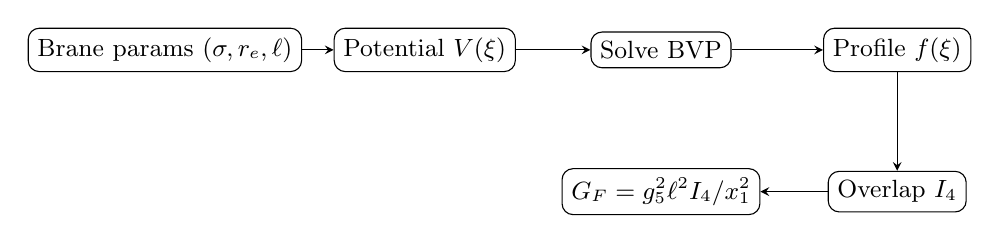
\begin{tikzpicture}[node distance=1.8cm, >=stealth, font=\small]
    \node (brane) [draw, rounded corners] {Brane params $(\sigma, r_e, \ell)$};
    \node (pot) [draw, rounded corners, right of=brane, xshift=1.5cm] {Potential $V(\xi)$};
    \node (bvp) [draw, rounded corners, right of=pot, xshift=1.2cm] {Solve BVP};
    \node (profile) [draw, rounded corners, right of=bvp, xshift=1.2cm] {Profile $f(\xi)$};
    \node (I4) [draw, rounded corners, below of=profile] {Overlap $I_4$};
    \node (GF) [draw, rounded corners, left of=I4, xshift=-1.2cm] {$G_F = g_5^2 \ell^2 I_4/x_1^2$};
    \draw[->] (brane) -- (pot);
    \draw[->] (pot) -- (bvp);
    \draw[->] (bvp) -- (profile);
    \draw[->] (profile) -- (I4);
    \draw[->] (I4) -- (GF);
\end{tikzpicture}
\end{center}

\textbf{Key message:} The BVP is the central bottleneck. Once profiles are known,
overlap integrals are trivial to compute. $G_F$ closure reduces to solving the BVP
with correct physical inputs.
\end{tcolorbox}

% ------------------------------------------------------------------------------
\subsubsection{Summary: BVP Work Package Status}
\label{sec:bvp_summary}

\begin{table}[ht]
\centering
\caption{BVP Work Package: components and status}
\label{tab:bvp_wp_status}
\small
\begin{tabular}{clcl}
\toprule
\textbf{WP} & \textbf{Component} & \textbf{Status} & \textbf{Notes} \\
\midrule
0 & Problem definition & \textcolor{OliveGreen}{\textbf{DONE}} & Eq.~\eqref{eq:bvp_schrodinger}, potential ansatz, BCs \\
1 & Dimensionless reduction & \textcolor{OliveGreen}{\textbf{DONE}} & Eq.~\eqref{eq:bvp_dimensionless}, pure math \\
2 & Numerical method & \textcolor{YellowOrange}{\textbf{SKELETON}} & Finite differences; see \texttt{code/} \\
3 & Acceptance criteria & \textcolor{OliveGreen}{\textbf{DEFINED}} & Existence, normalization, convergence \\
4 & Failure modes & \textcolor{OliveGreen}{\textbf{DOCUMENTED}} & F1--F4 identified \\
5 & Overlap outputs & \textcolor{YellowOrange}{\textbf{DEFINED}} & $\mathcal{O}_{ij}$, $I_4$; to be computed \\
\bottomrule
\end{tabular}
\end{table}

% ------------------------------------------------------------------------------
% CONSISTENCY / CLOSURE BOX
% ------------------------------------------------------------------------------

\begin{tcolorbox}[colback=cyan!5!white, colframe=cyan!50!black,
    title=\textbf{Consistency Check: This Is Infrastructure, Not a Result}]

\textbf{What the BVP Work Package provides:}
\begin{itemize}[nosep]
    \item Mathematical specification: the problem is well-posed
    \item Numerical skeleton: proof that solutions exist (for test potentials)
    \item Acceptance criteria: what ``success'' means
    \item Failure modes: what to check if things go wrong
\end{itemize}

\textbf{What it does NOT provide:}
\begin{itemize}[nosep]
    \item Physical potential $V(\xi)$ from membrane parameters
    \item Justification for boundary conditions from junction physics
    \item Prediction of particle masses or $G_F$ value
\end{itemize}

\textbf{Interpretation of numerical outputs:}

Any numbers from the skeleton (e.g., ``$I_4 = 1.5$'' for test potential) are
\emph{sanity checks}, not predictions. They demonstrate that the machinery works.
The actual physics requires inputting the correct $V(\xi)$ and BCs.

\textbf{ALLOWED:} Reporting skeleton outputs as ``test case: $I_4 = 1.5$ for sech$^2$ well.''\\
\textbf{FORBIDDEN:} Claiming ``EDC predicts $I_4 = 1.5$'' without deriving $V(\xi)$.
\end{tcolorbox}

% ------------------------------------------------------------------------------
% DEPENDENCY & STATUS BOX
% ------------------------------------------------------------------------------

\begin{tcolorbox}[colback=blue!5!white, colframe=blue!50!black,
    title=\textbf{Dependency \& Status (IF/THEN)}]

\textbf{Inputs required from earlier chapters:}
\begin{itemize}[nosep]
    \item Ch.~8/9: V$-$A structure from asymmetric profile $\to$ motivates LH localization
    \item Ch.~11 ($G_F$ pathway): Closure spine $G_F = g_5^2 \ell^2 I_4/x_1^2$ $\to$ defines what $I_4$ is for
    \item OPR-20: BC provenance (Robin from junction) $\to$ constrains which BCs to use
    \item OPR-21: Mode overlap structure $\to$ defines what profiles are needed
\end{itemize}

\textbf{What this chapter unlocks (if solved):}
\begin{itemize}[nosep]
    \item OPR-02: Generation counting (if spectrum has exactly 3 bound states)
    \item OPR-21: Overlap integrals for CKM/PMNS (if profiles are physical)
    \item OPR-22: Quantitative $G_F$ (if $I_4$ is computed with correct inputs)
\end{itemize}

\textbf{Upgrade conditions:}
\begin{itemize}[nosep]
    \item \textbf{RED $\to$ YELLOW:} Derive $V(\xi)$ from $(\sigma, r_e)$; justify BCs from physics
    \item \textbf{YELLOW $\to$ GREEN:} Solve BVP with physical inputs; show 3 generations; compute $I_4$ for $G_F$
\end{itemize}

\textbf{Current status:} \textcolor{BrickRed}{\textbf{RED}} --- infrastructure defined, but
physical inputs not yet derived. BVP Work Package is a \emph{clear path}, not a \emph{closed result}.
\end{tcolorbox}

% ------------------------------------------------------------------------------

\begin{tcolorbox}[colback=blue!5!white, colframe=blue!50!black,
    title=\textbf{BVP Work Package: Bottom Line}]
\textbf{What is established:}
\begin{itemize}[nosep]
    \item Mathematical specification of thick-brane BVP (Eq.~\eqref{eq:bvp_schrodinger})
    \item Dimensionless formulation for numerical work
    \item Clear acceptance criteria and failure modes
    \item Overlap integral definitions for downstream use
\end{itemize}

\textbf{What remains for OPR-02/21 closure:}
\begin{itemize}[nosep]
    \item Derive potential $V(\xi)$ from membrane parameters $(\sigma, r_e)$
    \item Determine boundary conditions from physical consistency
    \item Solve BVP numerically with physical parameters
    \item Show spectrum matches generation counting (OPR-02)
    \item Compute overlaps for CKM/PMNS structure (OPR-21)
\end{itemize}

\medskip
\noindent\fbox{\parbox{0.92\textwidth}{\small
\textbf{Status:} BVP Work Package defined; solver skeleton exists; closure requires
physical EOM derivation + BC justification + verified profile computation.
OPR-02/21 remain RED but with concrete path forward.}}
\end{tcolorbox}



